\section{Практическая часть}

\subsection{Задание 2. Исследование зон генерации}

Рабочий режим клистрона подбирался путем изменения напряжений на резонаторе (\(U_{\text{рез}}\)), ускоряющем электроде (\(U_{\text{уск}}\)) и отражателе (\(U_{\text{отр}}\)). Значения напряжений, при которых наблюдались три зоны генерации:
\begin{itemize}
	\item \(U_{\text{отр}} = 39\) В
	\item \(U_{\text{уск}} = 150\) В
	\item \(U_{\text{рез}} = 162\) В
\end{itemize}

Получим на экране осциллографа одну широкую зону. 
\begin{itemize}
	\item \(U_{\text{отр}} = 132\) В
	\item \(U_{\text{уск}} = 171\) В
	\item \(U_{\text{рез}} = 162\) В
\end{itemize}
Ширина частотной перестройки для одной зоны генерации составила: \(\Delta\lambda = 10.62 - 10.53 = 0.09\) см;

\subsection{Задания 3а и 4а}

Сняты зависимости тока детектора \(I\) и длины волны \(\lambda\) от напряжения на отражателе \(U_{\text{отр}}\) при фиксированных напряжениях на резонаторе. Измерения проводились в пределах зон генерации, полученных в задании 2. Результаты измерений представим в виде таблиц:

\begin{table}[h!]
	\centering
	\footnotesize
	\begin{tabular}{|l|c|c|c|c|c|c|c|c|c|c|c|c|c|}
		\hline
		\(U_{\text{отр}}\) & 2 & 6 & 7 & 10 & 12 & 14 & 16 & 18 & 29 & 30 & 36 & 39 & 40  \\ \hline
		\(I\), дел. & 0 & 5 & 0 & 0 & 25 & 27 & 20 & 0 & 0 & 17 & 32 & 17 & 0 \\ \hline
		\(\lambda\) & -- & 10.54 & -- & -- & 10.61 & 10.58 & 10.54 & -- & -- & 10.62 & 10.57 & 10.54 & -- \\ \hline
	\end{tabular}
	\caption{(опт) \(U_{\text{рез}} = 120\)}
\end{table}

\begin{table}[h!]
	\centering
	\footnotesize
	\begin{tabular}{|l|c|c|c|c|c|c|c|c|c|c|c|c|c|c|}
		\hline
		\(U_{\text{отр}}\) & 11 & 12 & 14 & 16 & 17 & 20 & 29 & 30 & 31 & 32 & 33 & 35 & 36 & 37  \\ \hline
		\(I\), дел. & 0 & 10 & 20 & 15 & 5 & 0 & 0 & 19 & 27 & 29 & 24 & 30 & 28 & 0  \\ \hline
		\(\lambda\) & -- & 10.60 & 10.58 & 10.54 & 10.53 & -- & -- & 10.60 & 10.60 & 10.59 & 10.58 & 10.57 & 10.56 & -- \\ \hline
	\end{tabular}
	\caption{(опт - 20V) \(U_{\text{рез}} = 100\)}
\end{table}

\begin{table}[h!]
	\centering
	\footnotesize
	\begin{tabular}{|l|c|c|c|c|c|c|c|c|c|c|c|c|c|c|c|c|}
		\hline
		\(U_{\text{отр}}\) & 2 & 3 & 4 & 5 & 6 & 10 & 11 & 12 & 13 & 14 & 15 & 16 & 18 & 32 & 34 & 37 \\ \hline
		\(I\), дел. & 0 & 7 & 8 & 8 & 0 & 0 & 14 & 26 & 27 & 21 & 23 & 22 & 0 & 0 & 30 & 20 \\ \hline
		\(\lambda\) & -- & 10.55 & 10.54 & 10.53 & -- & -- & 10.65 & 10.61 & 10.60 & 10.58 & 10.57 & 10.56 & -- & -- & 10.6 & 10.35 \\ \hline
	\end{tabular}
	\caption{(опт + 20V) \(U_{\text{рез}} = 140\)}
\end{table}

\vspace{0.5cm}

\begin{figure}[H]
	\centering
	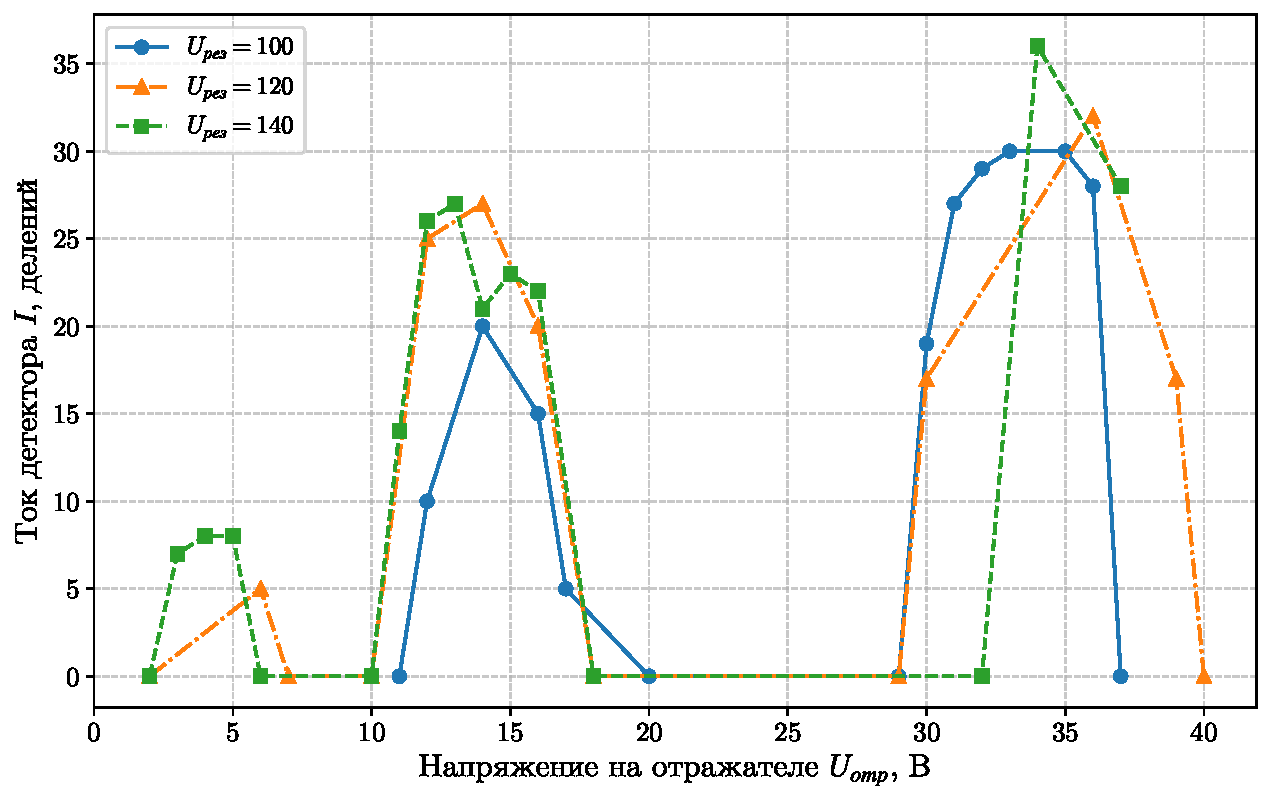
\includegraphics[angle = 0, width=1\textwidth]{python/images/graph_task_a.pdf} 
	\caption{Зависимость тока детектора \(I\) от напряжения на отражателе \(U_{\text{отр}}\) при различных \(U_{\text{рез}}\)}
	\label{fig:graph-1}
\end{figure}

\vspace{0.5cm}

\begin{figure}[h]
	\centering
	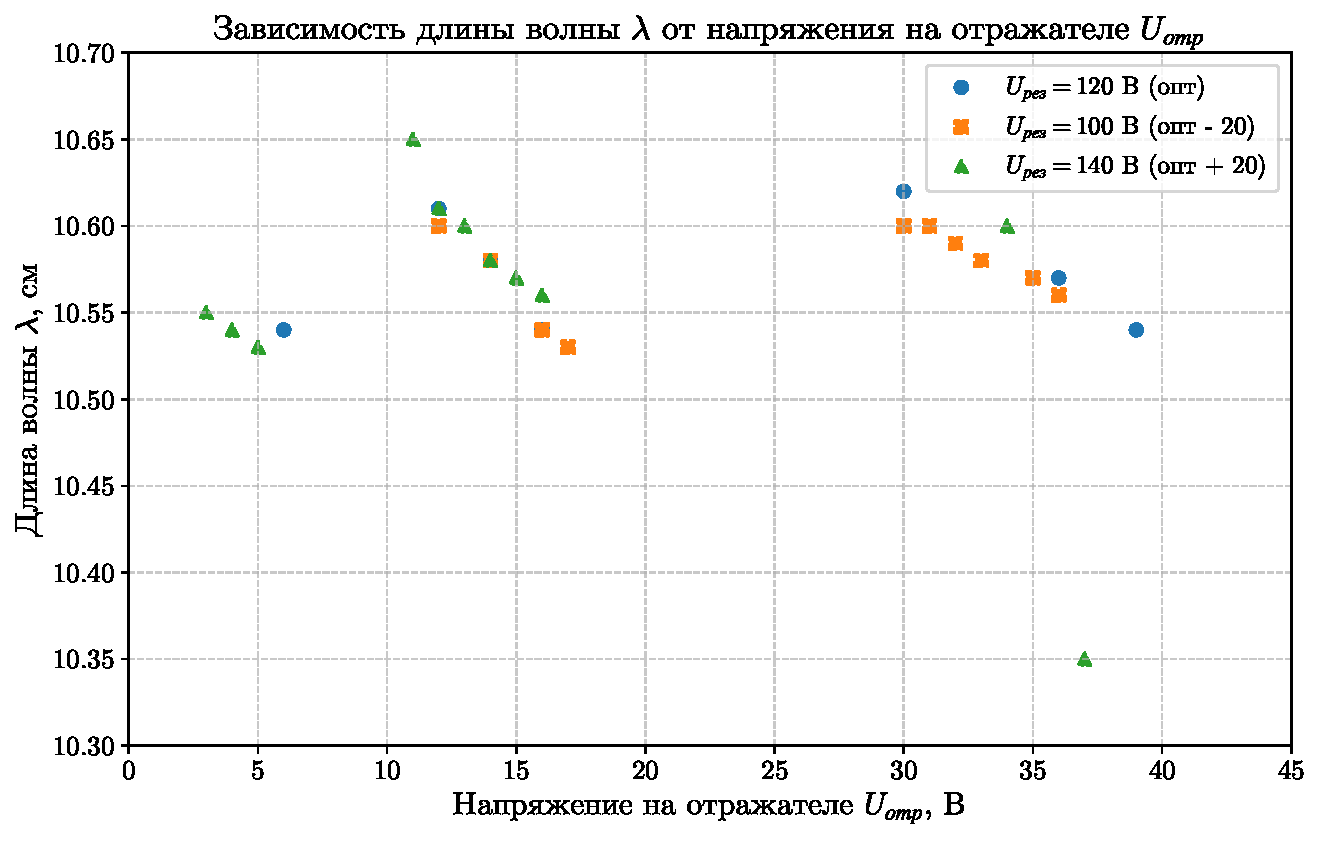
\includegraphics[angle = 0, width=1\textwidth]{python/images/graph_task_a_lambda.pdf} 
	\caption{Зависимость длины волны \(\lambda\) от напряжения на отражателе \(U_{\text{отр}}\) при различных \(U_{\text{рез}}\)}
	\label{fig:graph-a-lambda}
\end{figure}

\vspace{0.5cm}


\subsection{Задания 3б и 4б}

Сняты зависимости тока детектора \(I\) и длины волны \(\lambda\) от напряжения на резонаторе \(U_{\text{рез}}\) при фиксированных напряжениях на отражателе, соответствующих центрам зон генерации. Результаты измерений представим в таблицах

\begin{table}[h!]
	\centering
	\footnotesize
	\caption{Зависимость тока детектора \(I\) и длины волны \(\lambda\) от напряжения на резонаторе \(U_{\text{рез}}\) при \(U_{\text{отр}} = 42\) В}
	\begin{tabular}{|l|c|c|c|c|c|c|c|c|c|c|c|c|}
		\hline
		\(U_{\text{рез}}\), В & 20 & 25 & 30 & 35 & 40 & 45 & 50 & 55 & 60 & 65 & 70 & 75 \\ \hline
		\(I\), дел. & 0 & 7 & 17 & 23 & 28 & 29 & 28 & 29 & 29 & 28 & 18 & 0 \\ \hline
		\(\lambda\), см & -- & 10.58 & 10.58 & 10.58 & 10.58 & 10.58 & 10.56 & 10.55 & 10.54 & 10.52 & 10.50 & -- \\ \hline
	\end{tabular}
\end{table}

\vspace{0.5cm}

\begin{table}[h!]
	\centering
	\caption{Зависимость тока детектора \(I\) и длины волны \(\lambda\) от напряжения на резонаторе \(U_{\text{рез}}\) при \(U_{\text{отр}} = 108\) В}
	\begin{tabular}{|l|c|c|c|c|c|c|c|}
		\hline
		\(U_{\text{рез}}\), В & 30 & 40 & 50 & 60 & 70 & 80 & 90 \\ \hline
		\(I\), дел. & 0 & 25 & 30 & 30 & 32 & 31 & 2  \\ \hline
		\(\lambda\), см & -- & 10.56 & 10.57 & 10.5 & 10.57 & 10.56 & 10.56  \\ \hline
	\end{tabular}
\end{table}

\vspace{0.5cm}

\begin{figure}[h]
	\centering
	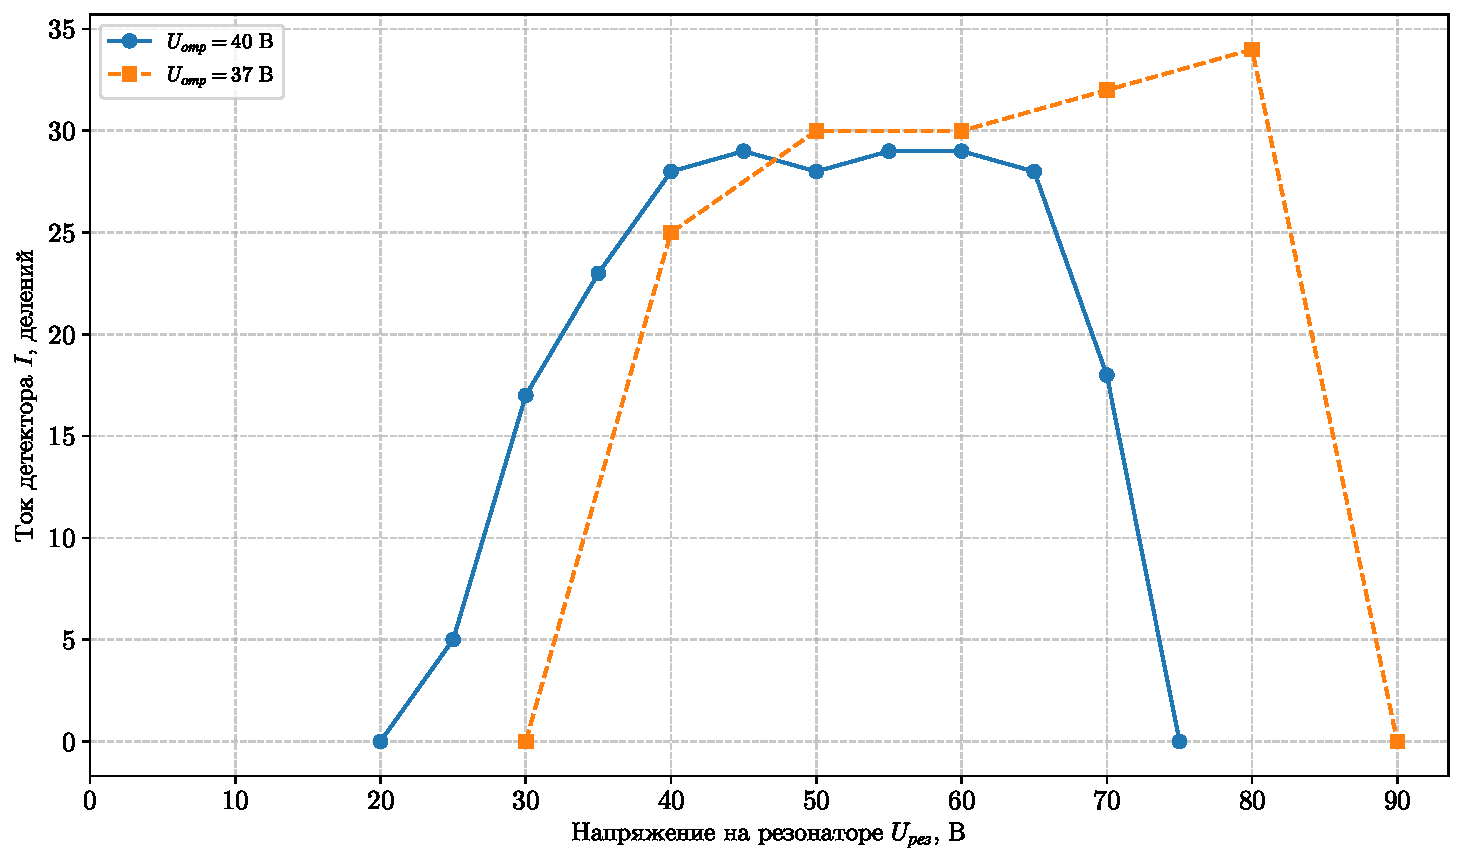
\includegraphics[angle = 0, width=1\textwidth]{python/images/graph_task_b.pdf} 
	\caption{Зависимости тока детектора \(I\)от напряжения на резонаторе \(U_{\text{рез}}\)}
	\label{fig:graph-2}
\end{figure}

\vspace{0.5cm}

\begin{figure}[h!]
	\centering
	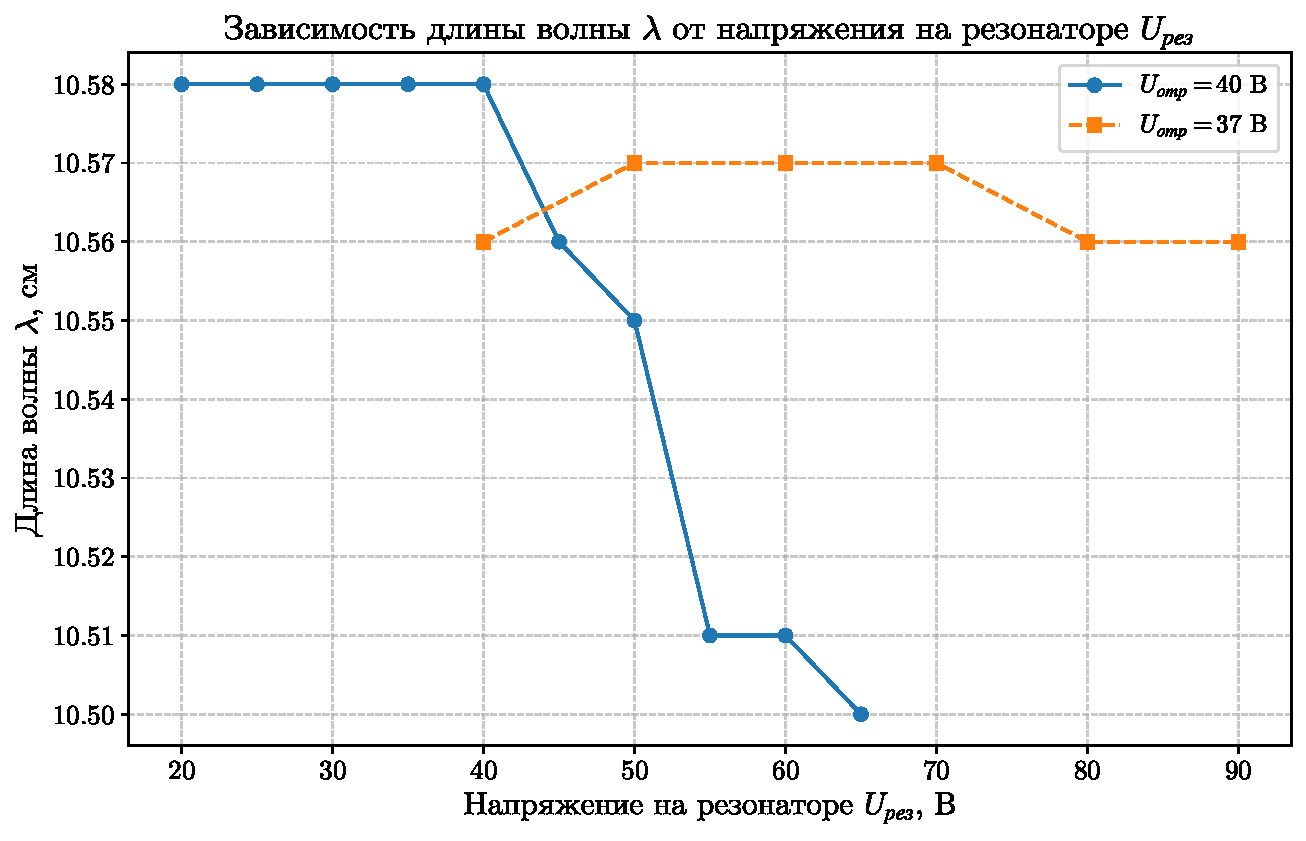
\includegraphics[angle = 0, width=1\textwidth]{python/images/graph_task_b_lambda.pdf} 
	\caption{Зависимость длины волны \(\lambda\) от напряжения на резонаторе \(U_{\text{рез}}\) при различных \(U_{\text{отр}}\)}
	\label{fig:graph-b-lambda}
\end{figure}

\vspace{0.5cm}

При увеличении абсолютной величины \(U_{\text{отр}}\) происходит рост частоты генерации клистрона.

\subsection{Задание 5}

Снята зависимость тока детектора \(I_{\text{д}}\) от тока пучка \(I_{\text{п}}\) для трех зон генерации. Потенциал отражателя для каждой зоны устанавливался по максимальной интенсивности колебаний. Регулировка тока пучка осуществлялась изменением напряжения на управляющем электроде. Результаты измерений приведём в виде таблиц.

\begin{table}[h!]
	\centering
	\caption{Зависимость тока детектора \(I_{\text{д}}\) от тока пучка \(I_{\text{п}}\), \(U_{\text{отр}} = 6\) В}
	\begin{tabular}{|l|c|c|c|c|c|c|c|c|c|c|c|c|}
		\hline
		\(I_{\text{п}}\), мА & 8 & 9 & 10 & 11 & 12 & 13 & 14 & 15 & 16 & 17 & 18 & 19 \\ \hline
		\(I_{\text{д}}\), дел. & 0 & 3 & 3 & 6 & 12 & 16 & 16 & 14 & 15 & 11 & 8 & 0 \\ \hline
	\end{tabular}
\end{table}

\vspace{0.5cm}

\begin{table}[h!]
	\centering
	\caption{Зависимость тока детектора \(I_{\text{д}}\) от тока пучка \(I_{\text{п}}\), \(U_{\text{отр}} = 14\) В}
	\begin{tabular}{|l|c|c|c|c|c|c|c|c|c|}
		\hline
		\(I_{\text{п}}\), мА & 13 & 14 & 15 & 16 & 17 & 18 & 19 & 20 & 21  \\ \hline
		\(I_{\text{д}}\), дел. & 0 & 3 & 22 & 23 & 24 & 24 & 24 & 22 & 22  \\ \hline
	\end{tabular}
\end{table}

\vspace{0.5cm}

\begin{table}[h!]
	\centering
	\caption{Зависимость тока детектора \(I_{\text{д}}\) от тока пучка \(I_{\text{п}}\), \(U_{\text{отр}} = 36\) В}
	\begin{tabular}{|l|c|c|c|c|c|c|c|}
		\hline
		\(I_{\text{п}}\), мА & 15 & 16 & 17 & 18 & 19 & 20 & 21 \\ \hline
		\(I_{\text{д}}\), дел. & 0 & 15 & 23 & 25 & 27 & 28 & 29 \\ \hline
	\end{tabular}
\end{table}
\vspace{0.5cm}
\begin{figure}[H]
	\centering
	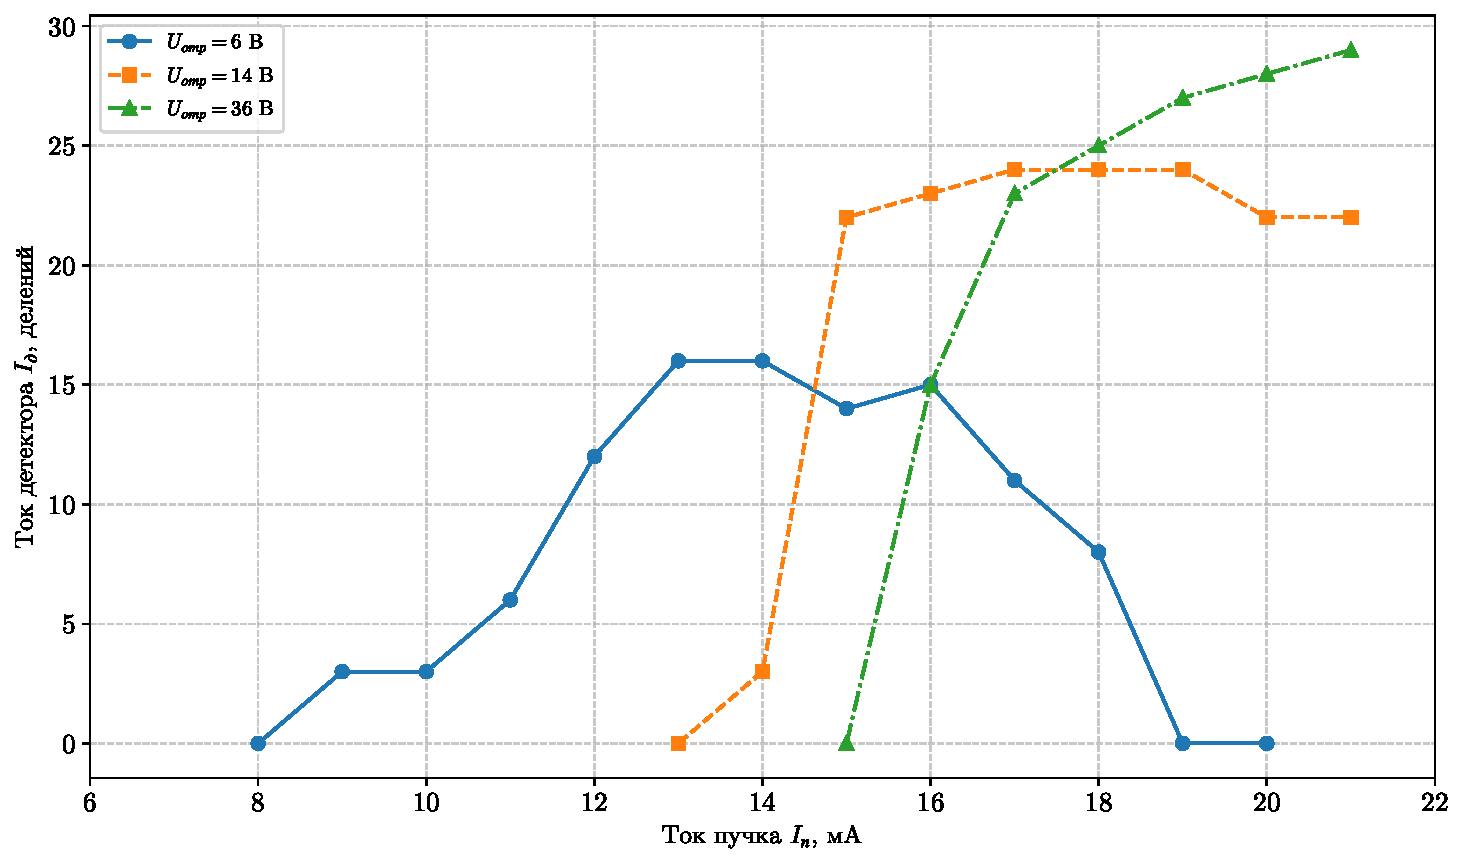
\includegraphics[angle = 0, width=1\textwidth]{python/images/graph_task_5.pdf} 
	\caption{Зависимость тока детектора \(I_{\text{д}}\) от тока пучка \(I_{\text{п}}\) при различных напряжениях на отражателе}
	\label{fig:graph-3}
\end{figure}

\vspace{0.5cm} 
